% Options for packages loaded elsewhere
\PassOptionsToPackage{unicode}{hyperref}
\PassOptionsToPackage{hyphens}{url}
%
\documentclass[
  ignorenonframetext,
]{beamer}
\usepackage{pgfpages}
\setbeamertemplate{caption}[numbered]
\setbeamertemplate{caption label separator}{: }
\setbeamercolor{caption name}{fg=normal text.fg}
\beamertemplatenavigationsymbolsempty
% Prevent slide breaks in the middle of a paragraph
\widowpenalties 1 10000
\raggedbottom
\setbeamertemplate{part page}{
  \centering
  \begin{beamercolorbox}[sep=16pt,center]{part title}
    \usebeamerfont{part title}\insertpart\par
  \end{beamercolorbox}
}
\setbeamertemplate{section page}{
  \centering
  \begin{beamercolorbox}[sep=12pt,center]{part title}
    \usebeamerfont{section title}\insertsection\par
  \end{beamercolorbox}
}
\setbeamertemplate{subsection page}{
  \centering
  \begin{beamercolorbox}[sep=8pt,center]{part title}
    \usebeamerfont{subsection title}\insertsubsection\par
  \end{beamercolorbox}
}
\AtBeginPart{
  \frame{\partpage}
}
\AtBeginSection{
  \ifbibliography
  \else
    \frame{\sectionpage}
  \fi
}
\AtBeginSubsection{
  \frame{\subsectionpage}
}
\usepackage{amsmath,amssymb}
\usepackage{iftex}
\ifPDFTeX
  \usepackage[T1]{fontenc}
  \usepackage[utf8]{inputenc}
  \usepackage{textcomp} % provide euro and other symbols
\else % if luatex or xetex
  \usepackage{unicode-math} % this also loads fontspec
  \defaultfontfeatures{Scale=MatchLowercase}
  \defaultfontfeatures[\rmfamily]{Ligatures=TeX,Scale=1}
\fi
\usepackage{lmodern}
\ifPDFTeX\else
  % xetex/luatex font selection
\fi
% Use upquote if available, for straight quotes in verbatim environments
\IfFileExists{upquote.sty}{\usepackage{upquote}}{}
\IfFileExists{microtype.sty}{% use microtype if available
  \usepackage[]{microtype}
  \UseMicrotypeSet[protrusion]{basicmath} % disable protrusion for tt fonts
}{}
\makeatletter
\@ifundefined{KOMAClassName}{% if non-KOMA class
  \IfFileExists{parskip.sty}{%
    \usepackage{parskip}
  }{% else
    \setlength{\parindent}{0pt}
    \setlength{\parskip}{6pt plus 2pt minus 1pt}}
}{% if KOMA class
  \KOMAoptions{parskip=half}}
\makeatother
\usepackage{xcolor}
\newif\ifbibliography
\setlength{\emergencystretch}{3em} % prevent overfull lines
\providecommand{\tightlist}{%
  \setlength{\itemsep}{0pt}\setlength{\parskip}{0pt}}
\setcounter{secnumdepth}{-\maxdimen} % remove section numbering
%\usetheme{metropolis}


%\setbeamercolor{normal text}{bg=white}
%\addtobeamertemplate{frametitle}{}{\vspace{-0.5em}} % decrease
%\setbeamersize{text margin left=5mm,text margin right=10mm}
%\usefonttheme[onlymath]{serif}
%\usefonttheme{professionalfonts}
%%%%%%%%%%%%%%%%
% Packages
%%%%%%%%%%%%%%%%

\usepackage{geometry}
\usepackage{graphicx}
\usepackage{amssymb}
\usepackage{amsopn}
\usepackage{cancel}
\usepackage{epstopdf}
\usepackage{amsmath}  	% this permits text in eqnarray among other benefits
\usepackage{url}		% produces hyperlinks
\usepackage{hyperref}	% allows for color usage in tables
\usepackage[english]{babel}
%\usepackage[latin1]{inputenc}
\usepackage{colortbl}	% allows for color usage in tables
\usepackage{multirow}	% allows for rows that span multiple rows in tables
\usepackage{color}		% this package has a variety of color options
\usepackage{xcolor}
\usepackage{pgf}
\usepackage{calc}
\usepackage{ulem}
\usepackage{multicol}
\usepackage{booktabs}
\usepackage{textcomp}
%\usepackage[misc]{ifsym} % for the dice symbol \Cube{}
%\usepackage{txfonts}
%\usepackage{listings}
%\usepackage{tikz}
\usepackage{array}
\usepackage{wasysym}
\usepackage{fancyvrb}

%% change fontsize of R code
\ifdefined\Shaded
\let\oldShaded\Shaded
\let\endoldShaded\endShaded
\renewenvironment{Shaded}{\footnotesize\oldShaded}{\endoldShaded}
\fi
%% change fontsize of output
\let\oldverbatim\verbatim
\let\endoldverbatim\endverbatim
\renewenvironment{verbatim}{\footnotesize\oldverbatim}{\endoldverbatim}

%%%%%%%%%%%%%%%%
% Remove navigation symbols
%%%%%%%%%%%%%%%%

\setbeamertemplate{navigation symbols}{}

\setbeamertemplate{footline}[frame number]

%%%%%%%%%%%%%%%%
% User defined colors
%%%%%%%%%%%%%%%%

\xdefinecolor{oiB}{rgb}{0.22,0.52,0.72}
\definecolor{oiG}{rgb}{.298,.447,.114}
\xdefinecolor{hlblue}{rgb}{0.051,0.65,1}
\xdefinecolor{gray}{rgb}{0.5, 0.5, 0.5}
\xdefinecolor{darkGray}{rgb}{0.3, 0.3, 0.3}
\xdefinecolor{darkerGray}{rgb}{0.2, 0.2, 0.2}
\xdefinecolor{rubineRed}{rgb}{0.89,0,0.30}
\xdefinecolor{irishGreen}{rgb}{0,0.60,0}	
\definecolor{lightGreen}{rgb}{0.387,0.581,0.148}

%%%%%%%%%%%%%%%%
% Template colors
%%%%%%%%%%%%%%%%

%\setbeamercolor*{palette primary}{fg=white,bg= oiB!80!black!90}
%\setbeamercolor*{palette secondary}{fg=black,bg= oiB!80!black}
%\setbeamercolor*{palette tertiary}{fg=white,bg= oiB!80!black!80}
%\setbeamercolor*{palette quaternary}{fg=white,bg= oiB}
%\setbeamercolor{structure}{fg= oiB}
%\setbeamercolor{frametitle}{bg= oiB!90}
%\setbeamertemplate{blocks}[shadow=false]
%\setbeamersize{text margin left=2em,text margin right=2em}

%\setbeamercolor{code body}{bg=gray!20!white!80,fg=black}


%%%%%%%%%%%%%%%%
% Get rid of fancy enumerated list bullets
%%%%%%%%%%%%%%%%

%\setbeamertemplate{enumerate items}[default]

%%%%%%%%%%%%%%%%
% Custom commands
%%%%%%%%%%%%%%%%

\newcommand{\Sum}{\sum\nolimits}
\newcommand{\Hide}[2]{\underline{~~~\onslide<#1>{\alert{#2}}~~~}}
\newcommand{\hide}[2]{\underline{~~\onslide<#1>{\alert{#2}}~~}}
\newcommand{\hid}[2]{\onslide<#1>{\alert{#2}}}
\newcommand{\code}[1]{\textcolor{blue}{\texttt{#1}}}

% red
\newcommand{\red}[1]{\textit{\textcolor{rubineRed}{#1}}}

% pink
\newcommand{\pink}[1]{\textit{\textcolor{rubineRed!90!white!50}{#1}}}

% green
\newcommand{\green}[1]{\textit{\textcolor{irishGreen}{#1}}}

% orange
\newcommand{\orange}[1]{\textit{\textcolor{orange}{#1}}}

% links: webURL, webLin, appLink
\newcommand{\webURL}[1]{\urlstyle{same}{ \textit{\textcolor{darkGray}{\url{#1}}}}}
\newcommand{\webLink}[2]{\href{#1}{\textcolor{darkGray}{{#2}}}}
\newcommand{\appLink}[2]{\href{#1}{\textcolor{white}{{#2}}}}

% mail
\newcommand{\mail}[1]{\href{mailto:#1}{\textit{\textcolor{darkGray}{#1}}}}

% highlighting: hl, hlGr, mathhl
\newcommand{\hl}[1]{\textit{\textcolor{hlblue}{#1}}}
\newcommand{\hlGr}[1]{\textit{\textcolor{lightGreen}{#1}}}
\newcommand{\mathhl}[1]{\textcolor{hlblue}{\ensuremath{#1}}}

% two col: two columns
\newenvironment{twocol}[4]{
\begin{columns}[c]
\column{#1\textwidth}
#3
\column{#2\textwidth}
#4
\end{columns}
}





%%%%%%%%%%%%%%%%
% Change margin
%%%%%%%%%%%%%%%%

\newenvironment{changemargin}[2]{%
\begin{list}{}{%
\setlength{\topsep}{0pt}%
\setlength{\leftmargin}{#1}%
\setlength{\rightmargin}{#2}%
\setlength{\listparindent}{\parindent}%
\setlength{\itemindent}{\parindent}%
\setlength{\parsep}{\parskip}%
}%
\item}{\end{list}}

%%%%%%%%%%%%%%%%
% Footnote
%%%%%%%%%%%%%%%%

\long\def\symbolfootnote[#1]#2{\begingroup%
\def\thefootnote{\fnsymbol{footnote}}\footnote[#1]{#2}\endgroup}

%%%%%%%%%%%%%%%%
% Graphics
%%%%%%%%%%%%%%%%

\DeclareGraphicsRule{.tif}{png}{.png}{`convert #1 `dirname #1`/`basename #1 .tif`.png}



\setbeamercolor{normal text}{bg=white}

\DeclareMathOperator{\var}{var}
\newcommand{\boxmodel}[1]{\begin{array}{|c|}#1\\[2pt]\hline\end{array}}
\newcommand{\BXX}[2]{\begin{array}{|@{\,}c@{\,}|@{\,}c@{\,}|}\hline#1&#2\\[-1pt]\hline\end{array}}
\newcommand{\p}{\mathrm{P}}
\newcommand{\SE}{\mathrm{SE}}
\newcommand{\xbar}{\overline{x}}
\newcommand{\Xbar}{\overline{X}}
\newcommand{\ybar}{\overline{y}}
\newcommand{\Ybar}{\overline{Y}}
\newcommand{\zbar}{\overline{z}}
\newcommand{\Zbar}{\overline{Z}}
\newcommand{\wbar}{\overline{w}}
\newcommand{\Wbar}{\overline{W}}
\newcommand{\vbar}{\overline{v}}
\newcommand{\Vbar}{\overline{V}}
\newcommand{\dbar}{\overline{d}}
\newcommand{\Dbar}{\overline{D}}
\newcommand{\ebar}{\overline{e}}
\newcommand{\ehat}{\widehat{\epsilon}}
\newcommand{\yhat}{\widehat{y}}
\newcommand{\Yhat}{\widehat{Y}}
\newcommand{\bhat}{\widehat{\beta}}
\newcommand{\dl}[1]{\widehat{\delta}_{#1}}
\newcommand{\g}[1]{\widehat{\gamma}_{#1}}
\newcommand{\al}[1]{\widehat{\alpha}_{#1}}
\newcommand{\Bj}{{\beta_j}}
\newcommand{\Bp}{{\beta_p}}
\newcommand{\Bq}{{\beta_q}}
\renewcommand{\b}[1]{\widehat{\beta}_{#1}}
\newcommand{\B}[1]{{\beta}_{#1}}
\newcommand{\BETA}{{\boldsymbol\beta}}
\newcommand{\bp}{\widehat{\beta}_p}
\newcommand{\bq}{\widehat{\beta}_q}
\newcommand{\bj}{\widehat{\beta}_j}
\newcommand{\df}{\mathrm{df}}
\DeclareMathOperator{\VIF}{VIF}
\DeclareMathOperator{\SSE}{SSE}
\DeclareMathOperator{\SST}{SST}
\DeclareMathOperator{\SSR}{SSR}
\DeclareMathOperator{\MSE}{MSE}
\DeclareMathOperator{\MST}{MST}
\DeclareMathOperator{\MSR}{MSR}
\DeclareMathOperator{\RM}{RM}
\DeclareMathOperator{\FM}{FM}
\DeclareMathOperator{\E}{E}
\DeclareMathOperator{\SD}{SD}
\DeclareMathOperator{\se}{se}
\DeclareMathOperator{\cov}{Cov}
\DeclareMathOperator{\corr}{Corr}
\DeclareMathOperator{\cor}{Cor}
\DeclareMathOperator{\Var}{Var}
\DeclareMathOperator{\logit}{logit}
\newcommand{\hsigma}{\widehat{\sigma}}
\newcommand{\betahat}{\widehat{\beta}}
\newcommand{\slide}{<br><br><br><br><br>}
\newcommand{\bbeta}{\boldsymbol{\beta}}
\newcommand{\bX}{\mathbf{X}}
\newcommand{\bY}{\mathbf{Y}}
\newcommand{\bH}{\mathbf{H}}
\newcommand{\bI}{\mathbf{I}}
\newcommand{\be}{\mathbf{e}}
\newcommand{\pval}{\mathit{P}\mathrm{-val}}



\newcommand{\vmu}{\mbox{\boldmath{$\mu$}}}
\newcommand{\vR}{\mbox{\boldmath{$R$}}}
\newcommand{\vpsi}{\mbox{\boldmath{$\psi$}}}
\newcommand{\vZ}{\mbox{\boldmath{$Z$}}}
\newcommand{\vX}{\mbox{\boldmath{$X$}}}
\newcommand{\vY}{\mbox{\boldmath{$Y$}}}
\newcommand{\vW}{\mbox{\boldmath{$W$}}}
\newcommand{\vz}{\mbox{\boldmath{$z$}}}
\newcommand{\vr}{\mbox{\boldmath{$r$}}}
\newcommand{\vx}{\mbox{\boldmath{$x$}}}
\newcommand{\vk}{\mbox{\boldmath{$k$}}}
\newcommand{\vp}{\mbox{\boldmath{$p$}}}
\newcommand{\vv}{\mbox{\boldmath{$v$}}}
\newcommand{\vg}{\mbox{\boldmath{$g$}}}
\newcommand{\vbeta}{\mbox{\boldmath{$\beta$}}}
\newcommand{\vone}{\mbox{\boldmath{$1$}}}
\newcommand{\vep}{\mbox{\boldmath{$\epsilon$}}}
\newcommand{\veta}{\mbox{\boldmath{$\eta$}}}
\newcommand{\vl}{\mbox{\boldmath{$l$}}}
\newcommand{\ve}{\mbox{\boldmath{$e$}}}
\newcommand{\va}{\mbox{\boldmath{$a$}}}
\newcommand{\vb}{\mbox{\boldmath{$b$}}}
\newcommand{\vPsi}{\mbox{\boldmath{$\Psi$}}}
\DeclareMathOperator*{\V}{\mathbb{V}}


% geometry: topsep=0pt 
\ifLuaTeX
  \usepackage{selnolig}  % disable illegal ligatures
\fi
\IfFileExists{bookmark.sty}{\usepackage{bookmark}}{\usepackage{hyperref}}
\IfFileExists{xurl.sty}{\usepackage{xurl}}{} % add URL line breaks if available
\urlstyle{same}
\hypersetup{
  pdftitle={STAT 20000 Chapter 4, Part 2The Average and Standard Deviation},
  pdfauthor={Yibi HuangDepartment of StatisticsUniversity of Chicago},
  hidelinks,
  pdfcreator={LaTeX via pandoc}}

\title{STAT 20000 Chapter 4, Part 2\newline The Average and Standard
Deviation}
% \author{Yibi Huang\newline Department of Statistics\newline University
% of Chicago}
\date{}

\begin{document}
\frame{\titlepage}

\hypertarget{five-number-summary-boxplots}{%
\section{Five-Number Summary \&
Boxplots}\label{five-number-summary-boxplots}}

\begin{frame}{Histograms and Percentiles}
\protect\hypertarget{histograms-and-percentiles}{}
What is the \(25^{\rm th}\) percentile of a histogram?

\begin{center}
\includegraphics[width=1\linewidth]{ch04B_24spr_files/figure-beamer/unnamed-chunk-2-1} \end{center}

The point on the horizontal axis such that \textbf{25\%} of the area
under the histogram lies to the left of that point (and \textbf{75\%} to
the right).
\end{frame}

\begin{frame}{}
\protect\hypertarget{section}{}
What is the \(25^{\rm th}\) percentile for the cigarette
histogram?\newline (The class intervals include the right endpoint, but
not the left.)

\begin{center}
\includegraphics[width=1\linewidth]{ch04B_24spr_files/figure-beamer/unnamed-chunk-3-1} \end{center}

So the \(25^{\rm th}\) percentile is about \Hide{2-}{13}.

\onslide<3->{\alert{\begin{center}
1 out of 4 of them smoked 13 or fewer cigarettes per day.
\end{center}}}
\end{frame}

\begin{frame}{}
\protect\hypertarget{section-1}{}
Other percentiles are defined in a similar way.\newline E.g., the
\(95^{\rm th}\) percentile is the point on the horizontal axis such that
95\% of the area under the histogram lies to the left of it.

\medskip

Q: What is the \(50^{\rm th}\) percentile for the cigarette histogram?

\begin{center}
\includegraphics[width=0.9\linewidth]{ch04B_24spr_files/figure-beamer/unnamed-chunk-4-1} \end{center}

\begin{itemize}
\tightlist
\item
  \(50^{\rm th}\) percentile = \Hide{2-}{20}.
\item
  \Hide{3-}{1} out of \Hide{3-}{2} of these men smoked \Hide{3-}{20} or
  fewer cigarettes per day.
\end{itemize}
\end{frame}

\begin{frame}{Quartiles, IQR, Five-Number Summary}
\protect\hypertarget{quartiles-iqr-five-number-summary}{}
\begin{itemize}
\tightlist
\item
  \textbf{Quartiles} divide data into 4 even parts

  \begin{itemize}
  \tightlist
  \item
    \textbf{first quartile} \(\mathbf{Q_1}=\) 25th percentile: \newline
    25\% of data fall below it and 75\% above it
  \item
    \textbf{second quartile} \(\mathbf{Q_2}=\) median \(=\) 50th
    percentile
  \item
    \textbf{third quartile} \(\mathbf{Q_3}=\) 75th percentile\newline
    75\% of data fall below it and 25\% above it
  \end{itemize}
\end{itemize}

\begin{center}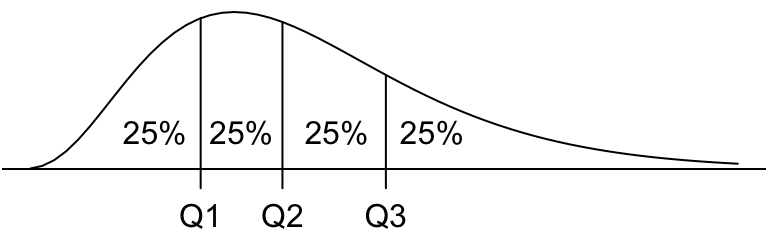
\includegraphics[width=0.65\linewidth]{ch04B_24spr_files/figure-beamer/quartiles-1} \end{center}

\vspace{-12pt}

\begin{itemize}
\tightlist
\item
  \textbf{Interquartile Range} \((IQR)=Q_3-Q_1\)
\item
  \textbf{Five-Number Summary}:
\end{itemize}

\begin{center}
    \begin{tabular}{ccccc}
      $\min,$ & $Q_1,$ & Median, & $Q_3,$ & $\max$
    \end{tabular}
\end{center}
\end{frame}

\begin{frame}{Example 1}
\protect\hypertarget{example-1}{}
For the 9 numbers: 43, 35, 43, 33, 38, 53, 64, 27, 34 \begin{align*}
&\begin{array}{c}
43\\
35\\
43\\
33
\end{array}\qquad
\left.\begin{array}{c}
27\\
\alert<3->{33}\\
\alert<3->{34}\\
35
\end{array}
\onslide<3->{\right\}
\alert{\leftarrow\begin{array}{c}\text{median}\\[-3pt]\text{of this half}\end{array}=\frac{33+34}{2}=33.5=Q_1}}\\[-8pt]
&\;\,38\;\;\stackrel{\text{sort}}{\longrightarrow}\;\,\structure<2->{38}\;\onslide<2->{\leftarrow\; \begin{array}{c}\text{overall}\\[-3pt]\text{median}\end{array}=Q_2}\\[-8pt]
&
\begin{array}{c}
53\\
64\\
27\\
34
\end{array}\qquad
\left.\begin{array}{c}
43\\
\alert<4->{43}\\
\alert<4->{53}\\
64
\end{array}\onslide<4->{\right\}\alert{\leftarrow\begin{array}{c}\text{median}\\[-3pt]\text{of this half}\end{array}=\frac{43+53}{2}=48=Q_3}}
\end{align*}

\begin{itemize}
\tightlist
\item
  IQR \(= Q_3-Q_1=48-33.5=14.5\)
\item
  Five number summary: 27, 33.5, 38, 48, 64
\end{itemize}
\end{frame}

\begin{frame}{Example 2}
\protect\hypertarget{example-2}{}
For the 10 numbers: 43, 35, 43, 33, 38, 53, 64, 27, 34, 27
\begin{align*}
\begin{array}{c}
43\\
35\\
43\\
33\\
38
\end{array}\qquad
\left.\begin{array}{c}
27\\ 27\\ \alert<3->{33}\\34\\ \structure<2->{35}
\end{array}\onslide<3->{\right\}&\alert{\leftarrow\begin{array}{c}\text{median}\\[-3pt]\text{of this half}\end{array}=33=Q_1}}\\[-17pt]
\stackrel{\text{sort}}{\longrightarrow}\quad\;\,\left.\begin{array}{c}\;\end{array}\right.&\onslide<2->{\leftarrow\; \begin{array}{c}\text{overall}\\[-3pt]\text{median}\end{array}=\frac{35+38}{2}=36.5=Q_2}\\[-17pt]
\begin{array}{c}
53\\
64\\
27\\
34\\
27
\end{array}\qquad
\left.\begin{array}{c}
\structure<2->{38}\\43\\ \alert<4->{43}\\ 53 \\64
\end{array}\onslide<4->{\right\}&\alert{\leftarrow\begin{array}{c}\text{median}\\[-3pt]\text{of this half}\end{array}=43=Q_3}}
\end{align*}

\begin{itemize}
\tightlist
\item
  IQR \(= Q_3-Q_1=43-33=10\)
\item
  Five number summary: 27, 33, 36.5, 43, 64
\end{itemize}
\end{frame}

\begin{frame}{Calculation of Quartiles}
\protect\hypertarget{calculation-of-quartiles}{}
Don't worry about the calculation of quartiles. Just keep in mind that

\begin{center}
\fbox{\fboxsep=6pt quartiles divide data into 4 even parts}
\end{center}
\end{frame}

\begin{frame}{Box-and-Whiskers Plot (also called Boxplot)}
\protect\hypertarget{box-and-whiskers-plot-also-called-boxplot}{}
\begin{minipage}{0.35\textwidth}
\textbf{1.5 IQR Rule}

Recall IQR $=$ Q3 $-$ Q1

observations that are
more than 1.5 IQR 
above Q3 or
below Q1 are (potential)
outleirs
\end{minipage}
\vspace{-1.3in}
\begin{flushright}
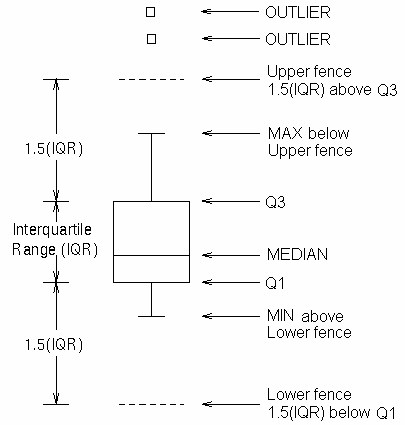
\includegraphics[width=0.65\textwidth]{boxplot.png}
\end{flushright}
\end{frame}

\begin{frame}{Boxplot v.s. Histogram --- Skewness}
\protect\hypertarget{boxplot-v.s.-histogram-skewness}{}
What does a boxplot look like if the histogram is symmetric?\pause

\begin{center}
\includegraphics[width=0.65\linewidth]{ch04B_24spr_files/figure-beamer/unnamed-chunk-5-1} \end{center}
\pause

Ditto, if right-skewed?\pause

\begin{center}
\includegraphics[width=0.65\linewidth]{ch04B_24spr_files/figure-beamer/unnamed-chunk-6-1} \end{center}
\end{frame}

\begin{frame}{Boxplot v.s. Histogram --- Modality}
\protect\hypertarget{boxplot-v.s.-histogram-modality}{}
Can you tell from a boxplot whether the distribution is unimodal or
bimodal?\pause

\begin{center}
\includegraphics[width=0.65\linewidth]{ch04B_24spr_files/figure-beamer/unnamed-chunk-7-1} \end{center}
\end{frame}

\hypertarget{back-to-fev-data}{%
\section{Back to FEV Data}\label{back-to-fev-data}}

\begin{frame}[fragile]{Example: FEV Data}
\protect\hypertarget{example-fev-data}{}
\small

The FEV data are data of a sample of 654 youths, aged 3 to 19, in the
area of East Boston during middle to late 1970's. The variables include

\begin{itemize}
\tightlist
\item
  \texttt{age}: subject's age in years
\item
  \texttt{fev}: lung capacity of subject, measured by \textbf{forced
  expiratory volume} (abbreviated as \textbf{FEV}), the amount of air an
  individual can exhale in the first second of forceful breath in liters
\item
  \texttt{ht}: subject's height in inches
\item
  \texttt{sex}: gender (0 = Female, 1 = Male)
\item
  \texttt{smoke}: smoking status (0 = Nonsmoker, 1 = Smoker)
\end{itemize}

\begin{verbatim}
  age   fev   ht sex smoke
    9 1.708 57.0   0     0
    8 1.724 67.5   0     0
    7 1.720 54.5   0     0
...(omitted)...
   15 3.211 66.5   0     0
\end{verbatim}
\end{frame}

\begin{frame}[fragile]{}
\protect\hypertarget{section-2}{}
Smokers had greater lung capacities than nonsmokers on average in the
FEV study. \red{Smoking increases one's lung capacity!?!}

\begin{verbatim}
    smoke   min    Q1 median    Q3   max     mean        sd   n
Nonsmoker 0.791 1.920  2.465 3.048 5.793 2.566143 0.8505215 589
   Smoker 1.694 2.795  3.169 3.751 4.872 3.276862 0.7499863  65
\end{verbatim}

\begin{center}
\includegraphics[width=0.8\linewidth]{ch04B_24spr_files/figure-beamer/unnamed-chunk-10-1} \end{center}

\begin{center}
\includegraphics[width=0.6\linewidth]{ch04B_24spr_files/figure-beamer/unnamed-chunk-11-1} \end{center}
\end{frame}

\begin{frame}{}
\protect\hypertarget{section-3}{}

\includegraphics[width=1\linewidth]{ch04B_24spr_files/figure-beamer/unnamed-chunk-12-1}
\end{frame}

\begin{frame}{Controlling for Confounders in Observational Studies}
\protect\hypertarget{controlling-for-confounders-in-observational-studies}{}
\begin{itemize}
\tightlist
\item
  Recall we can never make a \red{cause-and-effect} conclusion from an
  observational studies due to confounding
\item
  However, just because confounding is possible in observational studies
  does not mean that investigators are powerless to address it
\item
  Instead, well-conducted observational studies make strong efforts to
  identify confounders and \red{control for their effects}
\item
  There are many techniques for doing so; the most direct approach is to
  \red{make comparisons separately for smaller and
  more homogeneous groups}
\end{itemize}
\end{frame}

\begin{frame}{}
\protect\hypertarget{section-4}{}
\begin{itemize}
\tightlist
\item
  For example, studying the association between heart disease and
  smoking could be misleading, because men are more likely to have heart
  disease and also more likely to smoke
\item
  A solution is to compare heart disease rates separately for the two
  genders

  \begin{itemize}
  \tightlist
  \item
    male smokers v.s. male nonsmokers, and
  \item
    female smokers v.s. female nonsmokers
  \end{itemize}
\item
  Age is another common confounding factor that epidemiologists are
  often concerned with controlling for
\end{itemize}
\end{frame}

\begin{frame}{Is Gender a Confounder of the FEV Study?}
\protect\hypertarget{is-gender-a-confounder-of-the-fev-study}{}

\includegraphics[width=1\linewidth]{ch04B_24spr_files/figure-beamer/unnamed-chunk-13-1}
\end{frame}

\begin{frame}{}
\protect\hypertarget{section-5}{}
\begin{center}
\includegraphics[width=0.6\linewidth]{ch04B_24spr_files/figure-beamer/unnamed-chunk-14-1} \end{center}

\vspace{-10pt}

For females, did smokers or nonsmokers have greater lung
capacity?\newline How about males?
\end{frame}

\begin{frame}{Age Confounded Smoking Effect on Lung Capacities}
\protect\hypertarget{age-confounded-smoking-effect-on-lung-capacities}{}
\begin{center}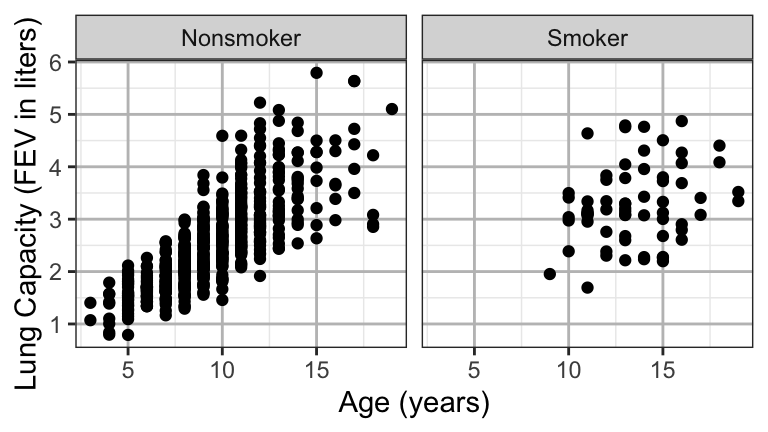
\includegraphics[width=0.8\linewidth]{ch04B_24spr_files/figure-beamer/age-fev-smoke-facets-1} \end{center}

\begin{itemize}
\tightlist
\item
  Older children had greater lung capacities
\item
  Smokers are older (mostly teens) while nonsmokers include children and
  teens
\end{itemize}
\end{frame}

\begin{frame}{Effect of Smoking on FEV After Accounting for Age}
\protect\hypertarget{effect-of-smoking-on-fev-after-accounting-for-age}{}

\includegraphics[width=1\linewidth]{ch04B_24spr_files/figure-beamer/unnamed-chunk-15-1}

\vspace{-12pt}

Considering children of the same age, did smokers or nonsmokers had
greater lung capacities in general?
\end{frame}

\begin{frame}{Effect of Smoking on FEV After Accounting for Age \& Sex}
\protect\hypertarget{effect-of-smoking-on-fev-after-accounting-for-age-sex}{}

\includegraphics[width=1\linewidth]{ch04B_24spr_files/figure-beamer/unnamed-chunk-16-1}
\end{frame}

\begin{frame}{Value of Observational Studies}
\protect\hypertarget{value-of-observational-studies}{}
\begin{itemize}[<+->]
\tightlist
\item
  It's possible to reveal the true relations between variables in
  observational studies, if we inspect the data carefully, controlling
  for potential confounding variables (making comparisons separately for
  each level of the confounding variable).
\item
  Carefully controlled observational studies can build up strong
  evidence for some ``cause-and-effect'' conclusions, though not
  conclusive.
\item
  Observational studies have tremendous value as initial studies to
  build up support for larger, more resource-intensive controlled
  experiments
\item
  However, they could be \hl{misleading} -- identifying confounders is
  not always easy, and you can't control for everything
\item
  Media often misinterpret association found in an scientific study as
  causation. Be cautious when reading news reports.
\end{itemize}
\end{frame}

\begin{frame}{Simpson's Paradox}
\protect\hypertarget{simpsons-paradox}{}
\red{Simpson's Paradox} is the phenomenon that a trend observed in
separate groups of data \alert{might} disappear or reverse when the
groups are combined.

\textbf{Example}: The FEV study is an example of Simpson's Paradox

\begin{itemize}
\tightlist
\item
  For each age group, nonsmokers had greater lung capacities in general
  than smokers
\item
  Combining all age groups, smokers had greater lung capacities in
  general than nonsmokers
\end{itemize}
\end{frame}

\begin{frame}{Example: Smoking and Longevity}
\protect\hypertarget{example-smoking-and-longevity}{}
A survey during 1972-74 recruited 1314 women in the United Kingdom and
asked if they smoked. A follow-up survey 20 years later determined
whether each woman was deceased or still alive.

\begin{center}
\begin{tabular}{@{}cccc@{}}
& Dead & Alive & Percentage Died\\\hline
Smoker    & 139 & 443 & $139/(139 + 443)\approx23.9\%$ \\
Nonsmoker & 230 & 502 & $230/(230 + 502)\approx31.4\%$\\\hline
\end{tabular}
\end{center}
\medskip

Surprisingly, smokers had a lower death rate than nonsmokers
\end{frame}

\begin{frame}{Example: Smoking and Longevity, Controlling for Age}
\protect\hypertarget{example-smoking-and-longevity-controlling-for-age}{}
\begin{center}\small
\begin{tabular}{@{}cccccc@{}}
Age in 1972  & Smoke? & Dead & Alive & Total & \% Dead\\\hline\hline
18-34 & Y & ~~5 & 174 & 179 & $5/179\approx2.8\%$ \\
      & N & ~~6 & 213 & 219 & $6/219\approx2.7\%$\\\hline
35-54 & Y & ~41 & 198 & 239 & $41/239\approx17.2\%$\\
      & N & ~19 & 180 & 199 & $19/199\approx9.5\%$\\\hline
55-64 & Y & ~51 & ~64 & 115 & $51/115\approx44.3\%$ \\
      & N & ~40 & ~81 & 121 & $40/121\approx33.1\%$\\\hline
65+   & Y & ~42 & ~~7 & ~49 & $42/49\approx85.7\%$\\
      & N & 165 & ~28 & 193 & $165/193\approx85.5\%$\\\hline
\end{tabular}
\end{center}

With each age group, smokers had a higher death rate than nonsmokers.

How could smokers have a lower death rate than nonsmokers when all age
groups are combined?
\end{frame}

\begin{frame}{Simpson's Paradox}
\protect\hypertarget{simpsons-paradox-1}{}
\vspace{-12pt}\begin{center}\small\tabcolsep=5pt
\begin{tabular}{@{}ccccccc@{}}
Age in 1972  & Smoke? & Dead & Alive & Total & \% Dead & \% Smoke \\\hline
18-34 & Y & ~~5 & 174 & 179 & ~2.8\% & \multirow{ 2}{*}{$\frac{179}{179+219}\approx45.0\%$}\\
      & N & ~~6 & 213 & 219 & ~2.7\%\\\hline
38-54 & Y & ~41 & 198 & 239 & 17.2\% & \multirow{ 2}{*}{$\frac{239}{239+199}\approx54.6\%$}\\
      & N & ~19 & 180 & 199 & ~9.5\%\\\hline
55-64 & Y & ~51 & ~64 & 115 & 44.3\% & \multirow{ 2}{*}{$\frac{115}{115+121}\approx48.7\%$}\\
      & N & ~40 & ~81 & 121 & 33.1\%\\\hline
65+   & Y & ~42 & ~~7 & ~49 & 85.7\% & \multirow{ 2}{*}{$\frac{49}{49+193}\approx20.2\%$}\\
      & N & 165 & ~28 & 193 & 85.5\%\\\hline
\end{tabular}
\end{center}

\begin{itemize}[<+->]
\tightlist
\item
  Old women (65+) were mostly dead 20 years later.
\item
  There were fewer smokers among old women
\item
  Smokers had a lower death rate because they were generally younger ---
  age is a confounder here.
\item
  \hl{Simpson's paradox}: a trend observed in different groups of data
  can disappear or reverse when the groups are combined.
\end{itemize}
\end{frame}

\begin{frame}{Sex Bias in Graduate Admissions}
\protect\hypertarget{sex-bias-in-graduate-admissions}{}
UC Berkeley admission rate:

\begin{center}
\begin{tabular}{@{}cccc@{}}
& Admitted & Rejected & Percentage Admitted\\\hline
Male   & 1198 & 1493 & $1198/(1198+1493)\approx44.5\%$ \\
Female &  557 & 1278 & $557/(557+1278)\approx30.4\%$\\\hline
\end{tabular}
\end{center}

\begin{itemize}
\tightlist
\item
  Sex bias?
\item
  The data is observational --- caution is in order.
\item
  This comparison is made over the whole university. Why not look at
  each individual department, which is smaller and more homogeneous?
\end{itemize}
\end{frame}

\begin{frame}{Sex Bias in Graduate Admissions (Cont'd)}
\protect\hypertarget{sex-bias-in-graduate-admissions-contd}{}
\begin{center}\small\tabcolsep=3pt
\begin{tabular}{@{}ccccccc@{}}
  & \multicolumn{3}{c}{Men} & \multicolumn{3}{c}{Women} \\\cmidrule(r){2-4}\cmidrule(l){5-7 }
  & Number & Number & Percent & Number & Number & Percent\\
Dept & Admitted & Rejected & Admitted & Admitted & Rejected & Admitted\\\midrule
A & 512& 313& 62\% & ~89 & ~19 & 82\%\\
B & 353& 207& 63\% & ~17 & ~~8 & 68\%\\
C & 120& 205& 37\% & 202 & 391 & 34\%\\
D & 138& 279& 33\% & 131 & 244 & 35\%\\
E & ~53& 138& 28\% & ~94 & 299 & 24\%\\
F & ~22& 351& ~6\% & ~24 & 317 & ~7\%\\\midrule
Total & 1198 & 1493 & 44.5\% & 557 & 1278 & 30.4\%
\end{tabular}
\end{center}

\textbf{Simpson's paradox}:

\begin{itemize}
\tightlist
\item
  In major A, admission rate: \textbf{female $>$ male}
\item
  In other majors, admission rate: \textbf{female $\approx$ male}
\item
  Overall admission rate: \textbf{female $<$ male}
\item
  Why is that?
\end{itemize}
\end{frame}

\begin{frame}{Sex Bias in Graduate Admissions (Cont'd)}
\protect\hypertarget{sex-bias-in-graduate-admissions-contd-1}{}
\begin{itemize}
\tightlist
\item
  More men apply for ``easy majors'' (A and B),\newline which raise the
  total number of admitted men, even though the admission rates for men
  are lower than women;
\item
  Most women applied for ``hard majors'' (C, D, E, F),\newline which
  lowers the total number of admitted women, even though the admission
  rates for women are roughly equal to men.
\item
  Confounding factor --- majors
\item
  Within-major comparisons lead to the correct conclusion. *A way to
  rule out the effect of a confounder is to \textbf{control for} it.
  That is, break the subjects by the confounder into groups, and make
  separate comparisons in all groups.
\end{itemize}
\end{frame}

\end{document}
